%%%%%%%%%%%%%%%%%%%%%%%%%%%%%%%%%%%%%%%%%%%%%%%%%%%%
% LECTURE 12
%%%%%%%%%%%%%%%%%%%%%%%%%%%%%%%%%%%%%%%%%%%%%%%%%%%%
\section*{Introduction to Convection}
\addcontentsline{toc}{section}{Introduction to Convection}
%%%%%%%%%%%%%%%%%%%%%%%%%%%%%%%%%%%%%%%%%%%%%%%%%%%%
\subsection*{The Nature of Convection}
\addcontentsline{toc}{subsection}{The Nature of Convection}
%%%%%%%%%%%%%%%%%%%%%%%%%%%%%%%%%%%%%%%%%%%%%%%%%%%%
Convection is the coupling between diffusion and motion:
\[
\text{Convection} = \text{Diffusion} + \text{Fluid Motion}
\]
%
In most heat rejection applications, fluid motion is crucial because it provides access to an effectively infinite heat sink (ambient air or flowing water). Unlike conduction problems, convection requires solving both the energy equation and fluid mechanics equations.
%%%%%%%%%%%%%%%%%%%%%%%%%%%%%%%%%%%%%%%%%%%%%%%%%%%%
\subsection*{Governing Equations for Convection}
\addcontentsline{toc}{subsection}{Governing Equations for Convection}
%%%%%%%%%%%%%%%%%%%%%%%%%%%%%%%%%%%%%%%%%%%%%%%%%%%%
\begin{definition}
The thermal energy equation for steady-state convection is:
\[
    \rho c_p \left(u\frac{\partial T}{\partial x} + v\frac{\partial T}{\partial y}\right) = k\nabla^2 T + \dot{q} + \mu\Phi
\]
%
Where $\mu\Phi$ represents viscous dissipation. For transient problems and when $k$ is not constant, we have:
\[
    \rho c_p \left[\frac{\partial T}{\partial t} + \mathbf{u}\cdot \nabla T\right] = \nabla \cdot(k\nabla T) + \dot{q} + \mu\Phi
\]
%
The viscous dissipation term $\mu\Phi$ in 2D is:
\[
    \mu\Phi = \mu\left\{2 \left[ 
    \left(\frac{\partial u}{\partial x}\right)^2 + \left(\frac{\partial v}{\partial y}\right)^2 \right] 
    + \left(\frac{\partial u}{\partial y} + \frac{\partial v}{\partial x}\right)^2\right\}
\]

This term is often negligible at low speeds but becomes important in high-shear applications like lubrication.
\end{definition}
%%%%%%%%%%%%%%%%%%%%%%%%%%%%%%%%%%%%%%%%%%%%%%%%%%%%
\subsection*{Boundary Layer Concept}
\addcontentsline{toc}{subsection}{Boundary Layer Concept}
%%%%%%%%%%%%%%%%%%%%%%%%%%%%%%%%%%%%%%%%%%%%%%%%%%%%
\subsubsection*{Velocity Boundary Layer}
\addcontentsline{toc}{subsubsection}{Velocity Boundary Layer}
%%%%%%%%%%%%%%%%%%%%%%%%%%%%%%%%%%%%%%%%%%%%%%%%%%%%
When uniform flow encounters a flat plate, a boundary layer develops:
\begin{itemize}
    \item At the surface, fluid velocity is zero (no-slip condition)
    \item The velocity gradually increases with distance from the surface
    \item At some distance $\delta$ from the surface, the velocity reaches 99\% of the free-stream velocity $u_\infty$
    \[
        u = 0.99 u_\infty
    \]
    \item The region where velocity transitions from 0 to $u_\infty$ is called the velocity boundary layer
    \item The boundary layer thickness $\delta$ increases with distance from the leading edge
\end{itemize}
%
\begin{figure}[H]
    \centering
    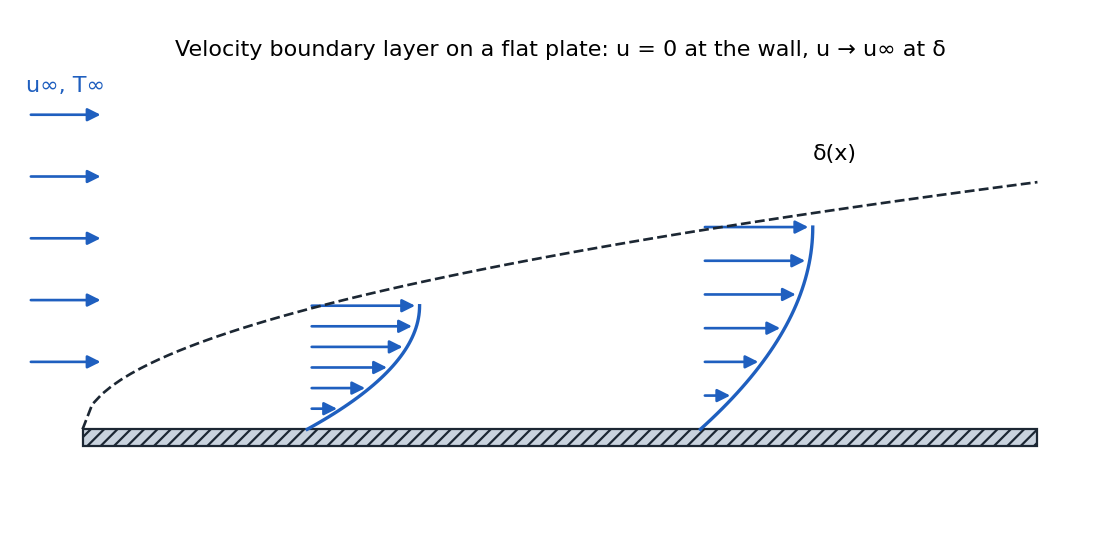
\includegraphics[width=0.7\linewidth]{pics/fig_2.png}
    \caption{Velocity boundary layer
development on a flat plate.}
\end{figure}
The wall shear stress is determined by the velocity gradient at the wall:
\[
\tau_s = \mu\left.\frac{\partial u}{\partial y}\right|_{y=0}
\]

Engineers often use a dimensionless friction coefficient:
\[
C_f = \frac{\tau_s}{\frac{1}{2}\rho\, u_\infty^2}
\]
%
\begin{figure}[H]
    \centering
    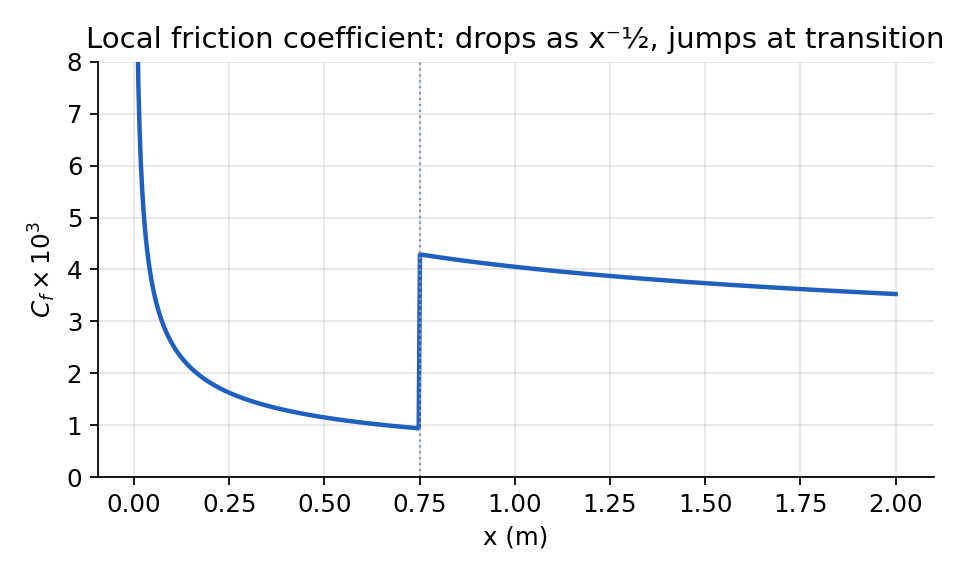
\includegraphics[width=0.5\linewidth]{pics/fig_5.png}
    \caption{Trends of $C_f$ and $\tau_s$ (similar to $\delta$ and $h$ for thermal boundary layers).}
    \label{fig::h_and_delta}
\end{figure}
%%%%%%%%%%%%%%%%%%%%%%%%%%%%%%%%%%%%%%%%%%%%%%%%%%%%%%%%%%5
\subsubsection*{Flow Regimes and Transitions}
\addcontentsline{toc}{subsubsection}{Flow Regimes and Transitions}
%%%%%%%%%%%%%%%%%%%%%%%%%%%%%%%%%%%%%%%%%%%%%%%%%%%%%%%%%%
The boundary layer can exist in three regimes:
\begin{itemize}
    \item \textbf{Laminar}: Near the leading edge, flow is smooth and ordered
    \item \textbf{Transition}: At some distance from the leading edge, instabilities develop
    \item \textbf{Turbulent}: Further downstream, the flow becomes fully turbulent with enhanced mixing
\end{itemize}
%
\begin{figure}[H]
    \centering
    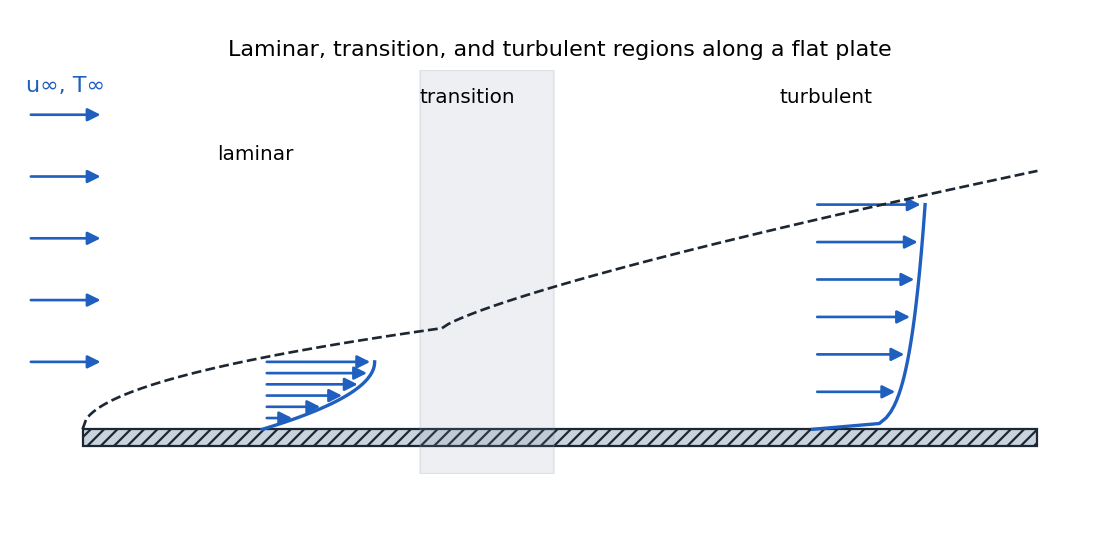
\includegraphics[width=0.7\linewidth]{pics/fig_3.png}
    \caption{Velocity boundary layer development on a flat plate.}
\end{figure}
%
In the transition region:
\begin{itemize}
    \item The boundary layer appears to thicken
    \item The wall shear stress increases
    \item Upon reaching fully turbulent flow, shear stress decreases again but remains higher than in the laminar region
\end{itemize}
%
\begin{figure}[H]
    \centering
    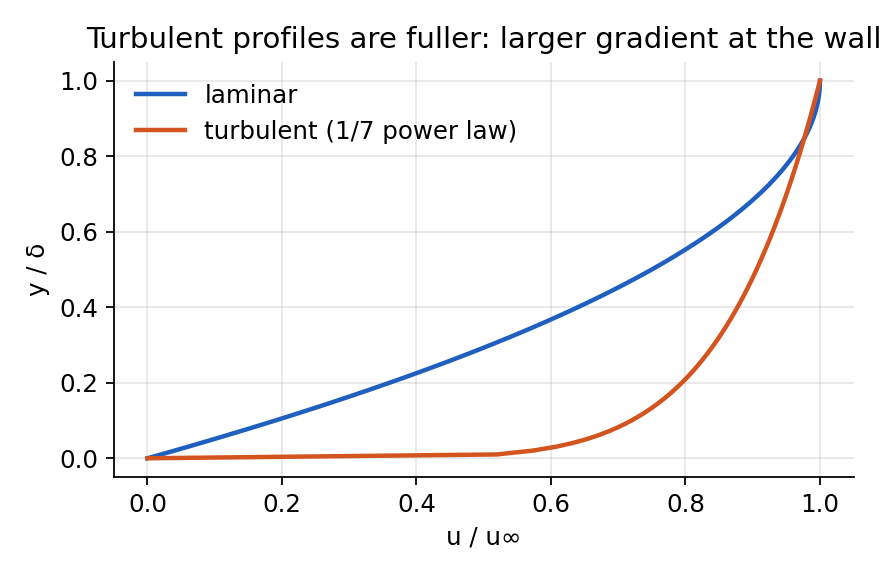
\includegraphics[width=0.5\linewidth]{pics/fig_4.png}
    \caption{Comparison of laminar and
turbulent velocity boundary layer profiles
for the same free stream velocity.}
\end{figure}
%
%%%%%%%%%%%%%%%%%%%%%%%%%%%%%%%%%%%%%%%%%%%%%%%%%%%%%%%%%%
\subsubsection*{Thermal Boundary Layer}
\addcontentsline{toc}{subsubsection}{Thermal Boundary Layer}
%%%%%%%%%%%%%%%%%%%%%%%%%%%%%%%%%%%%%%%%%%%%%%%%%%%%%%%%%%
When the plate temperature differs from the free-stream temperature, a thermal boundary layer develops:
\begin{itemize}
    \item At the wall, the temperature is $T_s$ (surface temperature)
    \item The temperature gradually transitions to $T_\infty$ (free-stream temperature)
    \item The thermal boundary layer thickness $\delta_T$ is defined where $(T_s-T)/(T_s-T_\infty) = 0.99$
    \item Like the velocity boundary layer, $\delta_T$ increases with distance from the leading edge
\end{itemize}
%
\begin{figure}[H]
    \centering
    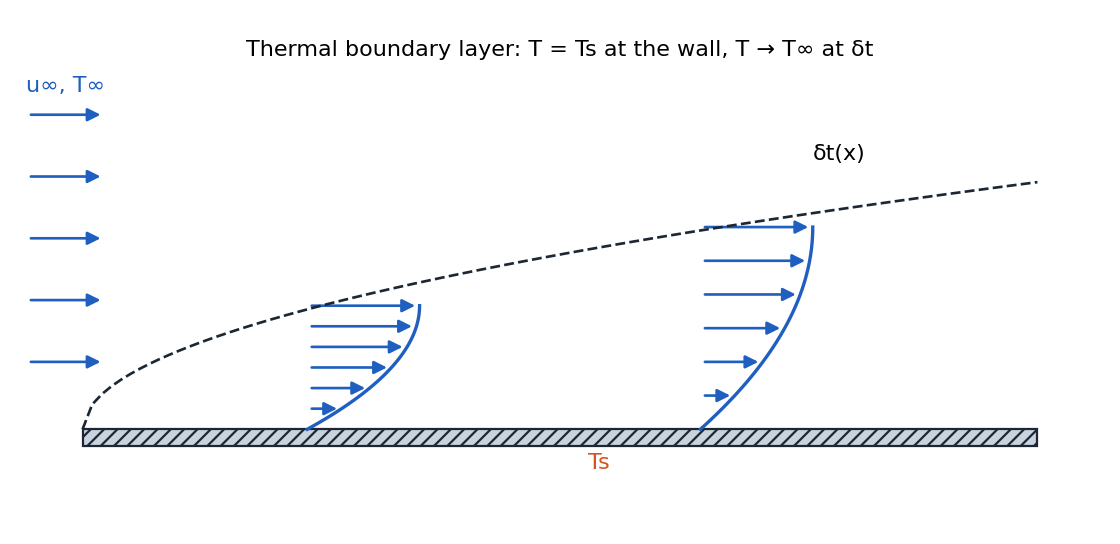
\includegraphics[width=0.7\linewidth]{pics/fig_6.png}
    \caption{Species concentration boundary
layer development on a flat plate.}
\end{figure}
%
The wall heat flux is determined by the temperature gradient at the wall:
%
\[
    q''_s = -k_f\left.\frac{\partial T}{\partial y}\right|_{y=0} = h_x(T_s-T_\infty)
\]
%
The local convection coefficient is defined as:
\[
    h = \frac{q''_s}{\underbrace{T_s - T_\infty}_{\Delta T}}
\]
%
In the laminar region, the convection coefficient decreases with distance from the leading edge. In the turbulent region, mixing enhances heat transfer, causing a significant increase in $h$ (The trend is shown in Fig. \ref{fig::h_and_delta})
%%%%%%%%%%%%%%%%%%%%%%%%%%%%%%%%%%%%%%%%%%%%%%%%%%%%
\subsubsection*{Concentration Boundary Layer}
\addcontentsline{toc}{subsubsection}{Concentration Boundary Layer}

Mass transport will not be our focus in this course, but it's important to understand the concept of concentration boundary layers, especially for those without previous exposure to mass transport.
%
\begin{figure}[H]
    \centering
    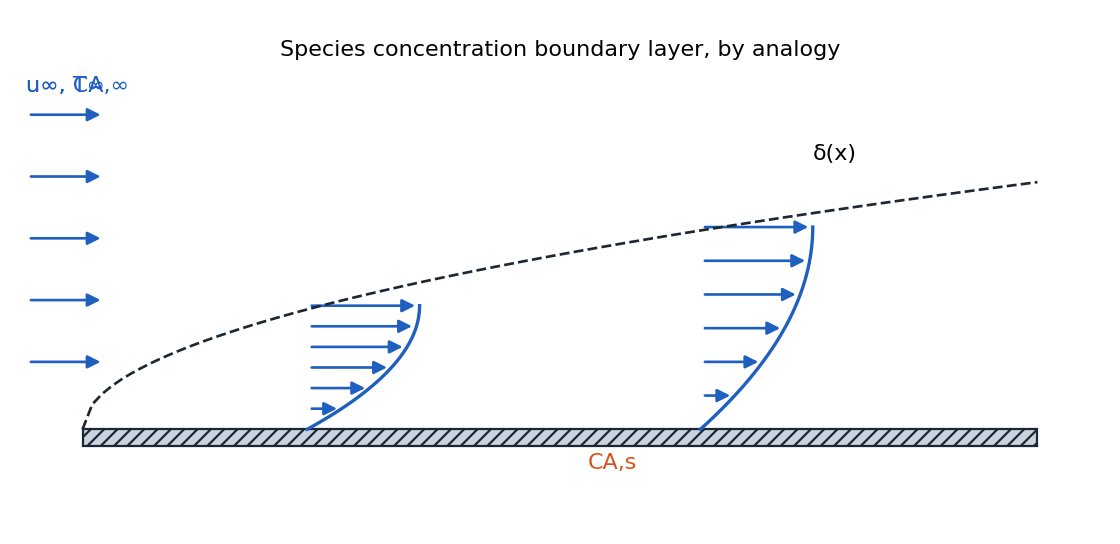
\includegraphics[width=0.6\linewidth]{pics/fig_7.png}
    \caption{Species concentration boundary
layer development on a flat plate.}
\end{figure}
%
Consider a surface with liquid water exposed to dry air (relative humidity less than 100\%):
\begin{itemize}
    \item At the surface, water vapor concentration reaches saturation ($C_{A,s}$)
    \item The surrounding air has a lower concentration ($C_{A,\infty}$)
    \item A gradient forms in the region adjacent to the surface
    \item Similar to velocity and thermal boundary layers, the concentration boundary layer is defined using the 99\% rule:
    \[
    \left[\left(C_{\mathrm{A}, s}-C_{\mathrm{A}}\right) /\left(C_{\mathrm{A}, s}-C_{\mathrm{A}, \infty}\right)\right]=0.99
    \]
\end{itemize}



This means the concentration boundary layer extends to the point where the concentration difference has decreased to 99\% of the total difference between the surface and free stream values.

The concentration at any point transitions from $C_{A,s}$ at the surface to $C_{A,\infty}$ in the free stream, with the boundary layer thickness ($\delta_m$) growing with distance from the leading edge in a similar shape to velocity and thermal boundary layers.
\\[0.5em]
The molar flux at the surface is governed by \textit{Fick's law }of diffusion:
\[
N''_A = -D_{AB}\left.\frac{\partial C_A}{\partial y}\right|_{y=0}
\]

Where:
\begin{itemize}
    \item $N''_A$ is the molar flux [kmol/(s·m$^2$)] or [kilo mole/(second·meter$^2$)]
    \item $D_{AB}$ is the binary diffusion coefficient [m$^2$/s]
    \item $C_A$ is the concentration of species A [kmol/m$^3$]
    \item $B$ is the matrix material and $A$ is the solution that dissolves inside
    \item $D_{AB}$ tells you how fast material $A$ can diffuse in solvent $B$
\end{itemize}

The convective mass transfer coefficient is defined as:
\[
h_m = \frac{N''_A}{\underbrace{C_{A,s} - C_{A,\infty}}_{\Delta C_A}}
\]

The unit of $h_m$ is [m/s], which is the same as velocity.
%
\paragraph{Why Boundary Layers Are Important?}
%
We put so much emphasis on boundary layers because they contain all the significant physics of heat transfer. The heat transfer between a surface and the surrounding fluid (at temperature $T_\infty$) occurs entirely within this thin layer. All the important gradients that drive heat transfer are confined to this region.


%%%%%%%%%%%%%%%%%%%%%%%%%%%%%%%%%%%%%%%%%%%%%%%%%%%%%%%%%%
\subsection*{Local and Average Convection Coefficient}
\addcontentsline{toc}{subsection}{Local and Average Convection Coefficient}
%%%%%%%%%%%%%%%%%%%%%%%%%%%%%%%%%%%%%%%%%%%%%%%%%%%%%%%%%%
In the first part of the course (conduction), we used Newton's law of cooling with a convection coefficient $h$. Now we can understand $h$ more precisely:
%
\begin{figure}[H]
    \centering
    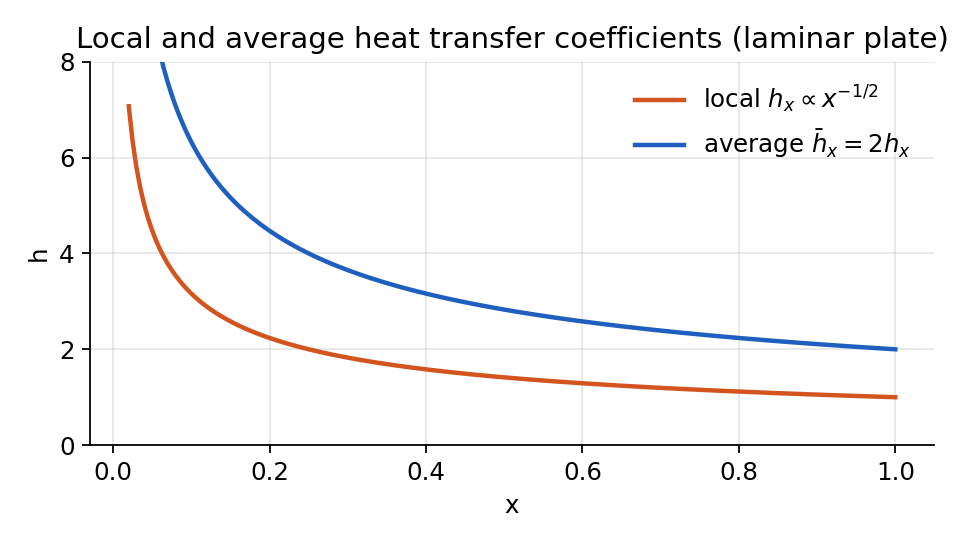
\includegraphics[width=0.7\linewidth]{pics/fig_8.png}
    \caption{Local and total
convection heat transfer. (a) Surface
of arbitrary shape. (b) Flat plate.}
\end{figure}
%
\begin{itemize}
    \item The local heat transfer coefficient $h_x$ at any point on a surface is defined as:
    \[
    h_x = \frac{q''_s}{T_s - T_\infty}
    \]
    where $q''_s$ is the local heat flux at that point.
    
    \item For the same object, the local $h$ can vary significantly from one location to another.
    
    \item The average heat transfer coefficient $\bar{h}$ is defined as:
    \[
    \bar{h} = \frac{1}{A_s}\int_{A_s} h_x\,dA_s
    \]
    
    \item This definition only works when $(T_s - T_\infty)$ is constant over the entire surface.
    \item $\bar{h}$ is what we use in Part 1 for conduction.
\end{itemize}

Similarly, for mass transfer, we can define an average mass transfer coefficient:
\[
    \begin{aligned}
        & N_A=\bar{h}_m A_S\left(C_{A, S}-C_{A, \infty}\right)
        \\[1em]
        & \bar{h}_m = \frac{1}{A_s}\int_{A_s} h_m\,dA_s
    \end{aligned}
\]

%%%%%%%%%%%%%%%%%%%%%%%%%%%%%%%%%%%%%%%%%%%%%%%%%%%%%%%%%%%
\subsubsection*{Mass Flux vs Molar Flux}
\addcontentsline{toc}{subsubsection}{Mass Flux Units}
%%%%%%%%%%%%%%%%%%%%%%%%%%%%%%%%%%%%%%%%%%%%%%%%%%%%%%%%%%%
In some cases, people use mass flux instead of molar flux:
\begin{itemize}
    \item Molar flux $N''_A$ [kmol/s·m$^2$] 
    \item Mass flux $n''_A$ [kg/s·m$^2$]
\end{itemize}

These are related by the molar mass. When using mass flux, the diffusion equation becomes:
\[
    \begin{aligned}
    & n_A^{\prime \prime}=h_m\left(\rho_{A, S}-\rho_{A, \infty}\right)\qquad \mathrm{[kg/s.m^2]}
    \\[1em]
    & n_A=h_m A_S\left(\rho_{A, S}-\rho_{A, \infty}\right)  \qquad \mathrm{[kg/s]}
    \\[1em]
    & n_{A, S}^{\prime \prime}=-\left.D_{A B} \frac{\partial \rho_A}{\partial y}\right|_{y=0}
    \end{aligned}
\]

where is $D_{AB}$ as before ($n''_{A}$: mass flux and $n_A$: mass transfer rate) and
\[
        h_m = \frac{n''_A}{\underbrace{\rho_{A, S}-\rho_{A, \infty}}_{\Delta \rho}}
\]
%%%%
\paragraph{Comparison}
The three transport processes (momentum, heat, and mass) can be analyzed using a unified framework:
% \begin{table}[H]
%     \centering
%     \begin{tabular}{m{4cm} m{4cm} m{4cm}}
%     Velocity & Thermal & Concentration 
%     \\ \toprule
%     $\tau_s= + \mu \frac{\partial u}{\partial y}\Bigl|_{y=0}$ & $q_s^{\prime \prime}=-\left.k \frac{\partial T}{\partial y}\right|_{y=0}$ & $N_A^{\prime \prime}=-D_{A B} \frac{\partial C_A}{\partial y}\Bigl|_{y=0}$ 
%     \\[1em]
%     $\delta$ & $\delta_t$ & $\delta_C$ 
%     \\[0.5em]
%     $\rho u_{\infty}$ & $T_{\infty}$ & $C_{A, \infty}$ 
%     \\[0.5em]
%     $\mu$ or $\nu$ & $k$ & $D_{A B}$ 
%     \\[0.5em]
%     $\tau_s$ & $q_s^{\prime \prime}$ & $N_A^{\prime \prime}$ 
%     \\[0.5em]
%     $C_f = \frac{\tau_s}{0.5\rho\,u_\infty}$ & $h=\frac{q_s^{\prime \prime}}{\Delta T}$ & $h_m = \frac{N''_A}{\Delta C}$ 
%     \\[1em]
%     $\Delta \dot{m} = \rho u_{\infty}-0$ & $\Delta T=T_s - T_\infty$ & $\Delta C_A = C_{A, S}-C_{A, \infty}$
%     \\ \bottomrule
%     \end{tabular}
% \end{table}
%%%
\begin{table}[H]
    \centering
    \begin{threeparttable}
        \begin{tabular}{m{4cm} m{4cm} m{4cm}}
            \toprule
            \textbf{Velocity} & \textbf{Thermal} & \textbf{Concentration} \\
            \midrule
            $\displaystyle \tau_w = \mu\left.\frac{\partial u}{\partial y}\right|_{y=0}$ & $\displaystyle q'' = -k\left.\frac{\partial T}{\partial y}\right|_{y=0}$ & $\displaystyle N_A'' = -D_{AB}\left.\frac{\partial C_A}{\partial y}\right|_{y=0}$ \\
            [1em]
            $\delta$ & $\delta_t$ & $\delta_c$ \\
            [0.5em]
            $U_{\infty}$ & $T_{\infty}$ & $C_{A,\infty}$ \\
            [0.5em]
            $\mu$ (or $\nu$) & $k$ & $D_{AB}$ \\
            [0.5em]
            $\tau_w$ & $q''$ & $N_A''$ \\
            [0.5em]
            $\displaystyle C_f = \dfrac{\tau_w}{\tfrac12 \rho U_{\infty}^{2}}$\tnote{\dag} & $\displaystyle h = \dfrac{q''}{\Delta T}$ & $\displaystyle h_m = \dfrac{N_A''}{\Delta C}$ \\
            [1em]
            $\Delta u = U_{\infty} - 0$ & $\Delta T = T_s - T_{\infty}$ & $\Delta C = C_{A,s} - C_{A,\infty}$ \\
            \bottomrule
        \end{tabular}
        \begin{tablenotes}\footnotesize
            \item[\dag] For momentum transfer the driving potential is the \emph{dynamic pressure} $\operatorname{P}_{d} = \tfrac12 \rho U_{\infty}^{2}$, analogous to $\Delta T$ and $\Delta C$ in heat and mass transfer.
        \end{tablenotes}
    \end{threeparttable}
\end{table}
%
While these three processes involve different physical quantities, they share the same mathematical structure because, at the microscopic level, they all result from the same random molecular motion. When molecules move randomly between regions, they simultaneously transport momentum, energy, and mass.
%%%%%%%%%%%%%%%%%%%%%%%%%%%%%%%%%%%%%%%%%%%%%%%%%%%%%%%%%%
\subsection*{Understanding Boundary Layers as Insulation Layers}
\addcontentsline{toc}{subsection}{Understanding Boundary Layers as Insulation Layers}
%%%%%%%%%%%%%%%%%%%%%%%%%%%%%%%%%%%%%%%%%%%%%%%%%%%%%%%%%%
It's crucial to understand that boundary layers act as insulation layers:
\\[1em]
$\left\{\begin{array}{l}
        \text { Velocity } 
        \\ 
        \text { Thermal } 
        \\ 
        \text { Concentration }
       \end{array}
\right\}$ 
BL is layer of \textbf{insulation for diffusion } of 
$\left\{\begin{array}{l}
    \text { Linear momentum } 
    \\ 
    \text { Thermal Energy } 
    \\ 
    \text { molecules. }
    \end{array}
\right\}$
driven by 
$\left\{\begin{array}{l}
        \text { surface shear } 
        \\ 
        \text { surface heat flux } 
        \\ 
        \text { surface molar flux}
        \end{array}\right\}
$.
\\[1em]
Key insight: \textbf{Thicker boundary layers lead to less transfer, not more.} This is sometimes counter-intuitive for newcomers to the field.
%%%%%%%%%%%%%%%%%%%%%%%%%%%%%%%%%%%%%%%%%%%%%%%%%%%%%%%%%%%
\subsection*{Microscopic View of Transport Phenomena}
\addcontentsline{toc}{subsection}{Microscopic View of Transport Phenomena}

The transport of momentum, energy, and mass occurs simultaneously at the molecular level:
\begin{itemize}
    \item Random molecular motion causes molecules to move between regions of different velocity, temperature, and concentration
    \item When molecules change positions, they carry their momentum, thermal energy, and identity
    \item This explains why the three transport phenomena follow similar mathematical forms
\end{itemize}

Consider a simple Couette flow between parallel plates:
\begin{itemize}
    \item Microscopically, molecules move randomly while maintaining a net velocity gradient
    \item This random motion transfers momentum from high-velocity regions to low-velocity regions
    \item The same mechanism transfers thermal energy and species concentration
\end{itemize}

\subsection*{Boundary Layer Equations}
\addcontentsline{toc}{subsection}{Boundary Layer Equations}

Based on experimental observations, in boundary layers $v \ll u$:
%

\begin{minipage}{0.3\textwidth}% adapt widths of minipages to your needs
%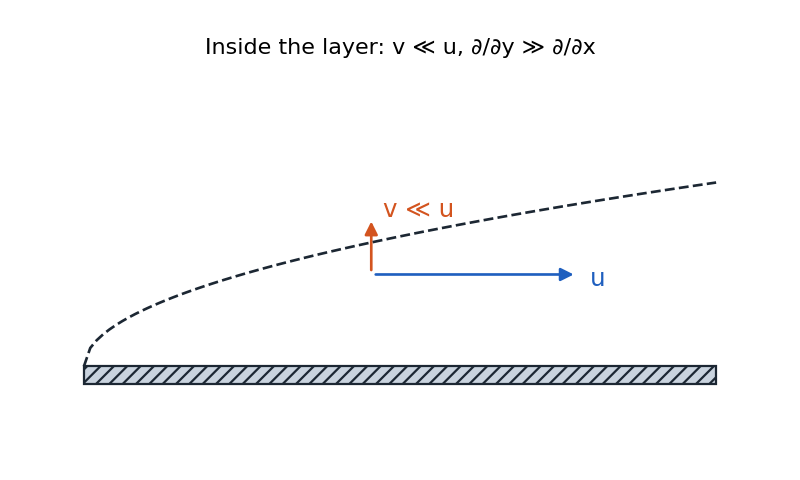
\includegraphics[width=1.3\linewidth]{pics/fig_9.png}
\begin{figure}[H]
    \centering
        \begin{tikzpicture}[xscale=1,yscale=1]
      % --- solid wall 
      \fill[pattern=north east lines, pattern color=black!60] (0,-0.2) rectangle (6,0);
      \draw[line width=0.3pt] (0,0) -- (6,0);

      % --- velocity boundary‑layer edge  delta
      \draw[dashed,line width=0.6pt] (0,0)
            .. controls (1,1.4) and (4,2.0) .. (6,2.4);

      % --- concentraion boundary‑layer edge  delta
      \draw[dashed,line width=0.6pt] (0,0)
            .. controls (1,1.0) and (4,1.6) .. (6,1.9);

      % --- thermal boundary‑layer edge delta
      \draw[dashed,line width=0.6pt] (0,0)
            .. controls (1,1.0) and (4,1.6) .. (6,1.9);
    
      % --- thermal boundary‑layer edge  delta_t
      \draw[dashed,line width=0.6pt] (0,0)
            .. controls (1,0.45) and (4,0.7) .. (6,0.85);
    
      % --- arrow showing delta_c
      \draw[<->,thick] (4,0) -- (4,1.4);
      \node[right] at (4,0.9) {$\delta_c$};
    
      % --- arrow showing delta_t
      \draw[<->,thick] (5,0) -- (5,0.75);
      \node[right] at (5,0.38) {$\delta_t$};

      % --- arrow showing delta
      \draw[<->,thick] (3,0) -- (3,1.7);
      \node[right] at (3,1.0) {$\delta$};

      % --- arrow showing x
      \draw[|->,thick] (0,-0.5) -- (0.6,-0.5);
      \node[right] at (0.07, -0.8) {$x$};
      
    \end{tikzpicture}
\end{figure}
\end{minipage}%
\hfill%
\begin{minipage}{0.6\textwidth}\raggedleft
\[
    \left\{\begin{array}{l}
    \frac{\partial^2 u}{\partial x^2} \ll \frac{\partial^2 u}{\partial y^2} 
    \\[1em]
    \frac{\partial^2 T}{\partial x^2} \ll \frac{\partial^2 T}{\partial y^2} 
    \\[1em]
    \frac{\partial^2 C_A}{\partial x^2} \ll \frac{\partial^2 C_A}{\partial y^2}
    \end{array}\right.
\]
\end{minipage}
%
The boundary layer equations are normalized by first defining dimensionless independent
variables of the forms:

\[
x^* = \frac{x}{L}, \quad y^* = \frac{y}{L}, \quad u^* = \frac{u}{U_\infty}, \quad v^* = \frac{v}{U_\infty}
\]
%
\[
    \begin{gathered}
    T^* \equiv \frac{T-T_s}{T_{\infty}-T_s} 
    \\[1em]
    C_{\mathrm{A}}^* \equiv \frac{C_{\mathrm{A}}-C_{\mathrm{A}, s}}{C_{\mathrm{A}, \infty}-C_{\mathrm{A}, s}}
    \end{gathered}
\]
%
\begin{table}[H]
\centering
\renewcommand{\arraystretch}{3.0}  % Increase vertical spacing (adjust value as needed)
\begin{tabular}{|c|c|cc|}
\hline
\multirow{2}{*}{Boundary Layer} & \multirow{2}{*}{Conservation Equation} & \multicolumn{2}{c|}{Boundary Conditions} 
\\
\cline{3-4}
 &  & Wall & Free Stream 
 \\
\hline
Velocity & $u^*\frac{\partial u^*}{\partial x^*} + v^*\frac{\partial u^*}{\partial y^*} = -\frac{dp^*}{dx^*} + \frac{1}{\operatorname{Re_L}}\frac{\partial^2 u^*}{\partial y^{*2}}$ & $u^*(x^*,0) = 0$ & $u^*(x^*,\infty) = 1$ 
\\
\hline
Thermal & $u^*\frac{\partial T^*}{\partial x^*} + v^*\frac{\partial T^*}{\partial y^*} = \frac{1}{\operatorname{Re_L} \,\operatorname{Pr}}\frac{\partial^2 T^*}{\partial y^{*2}}$ & $T^*(x^*,0) = 0$ & $T^*(x^*,\infty) = 1$ 
\\
\hline
Concentration & $u^*\frac{\partial C_A^*}{\partial x^*} + v^*\frac{\partial C_A^*}{\partial y^*} = \frac{1}{\operatorname{Re_L}\, \operatorname{Sc}}\frac{\partial^2 C_A^*}{\partial y^{*2}}$ & $C_A^*(x^*,0) = 0$ & $C_A^*(x^*,\infty) = 1$ 
\\
\hline
\end{tabular}
%\caption{Boundary Layer Equations and Conditions}
\end{table}
%
In other words,
\[
    \begin{array}{l}
         u^* = f_v\left(x^*,y^*,\operatorname{Re}, 1, \frac{dp^*}{dx^*}\right)  
         \\[1em]
         T^* = f_t\left(x^*,y^*,\operatorname{Re}, \operatorname{Pr}, \frac{dp*}{dx*}\right) 
         \\[1em]
         C^*_A = f_c\left(x^*,y^*,\operatorname{Re}, \operatorname{Sc}, \frac{dp*}{dx*}\right)          
    \end{array}
\]
%
\begin{table}[H]
    \centering
    \renewcommand{\arraystretch}{3}  % Increase vertical spacing
    \begin{tabular}{|c|c|}
    \hline
    Boundary Layer & Similarity Parameter(s) \\
    \hline
    Velocity & $\operatorname{Re}_L = \frac{\rho U L}{\mu}=\frac{U\, L}{\nu}$ \\
    \hline
    Thermal & $\operatorname{Re}_L, \operatorname{Pr} = \frac{\nu}{\alpha}$ \\
    \hline
    Concentration & $\operatorname{Re}_L, \operatorname{Sc} = \frac{\nu}{D_{AB}}$ \\
    \hline
    \end{tabular}
    %\caption{Similarity Parameters for Boundary Layer Equations}
\end{table}
%
\paragraph{Note} For a flat plate, $\frac{\partial p^*}{\partial x^*} = 0$ (zero pressure gradient).
\\[1em]
\textit{proof:} This may not sound intuitive, but can be explained using Bernoulli's equation:
\[
P + \rho gz + \frac{1}{2}\rho u^2 = \text{constant}
\]

For a flat plate flow, we can neglect the $\rho gz$ term. If we look at the flow just above the boundary layer, the velocity $u$ is constant ($u_\infty$), which means the dynamic pressure term $\frac{1}{2}\rho u^2$ is constant. Since the total is constant, the static pressure $P$ must also be constant, meaning $\frac{dp}{dx} = 0$.
\\[1em]
The boundary layer is actually extremely thin compared to how it's typically illustrated. If drawn to scale for a typical flow at 1 m/s, it would be barely visible. The thick representation is only for visualization purposes, to show that the layer exists.

%%%%%%%%%%%%%%%%%%%%%%%%%%%%%%%%%%%%%%%%%%%%%%%%%%%%%%%%%
\subsection*{Dimensionless Numbers}
\addcontentsline{toc}{subsection}{Dimensionless Numbers}
%%%%%%%%%%%%%%%%%%%%%%%%%%%%%%%%%%%%%%%%%%%%%%%%%%%%%%%%
\subsubsection*{Reynolds Number}
\addcontentsline{toc}{subsubsection}{Reynolds Number}
%%%%%%%%%%%%%%%%%%%%%%%%%%%%%%%%%%%%%%%%%%%%%%%%%%%%%%%%
\begin{definition}
    \[
        \operatorname{Re_L} = \frac{\rho\, U\,L}{\mu} =\frac{U\, L}{\mu/\rho} = \frac{U\,L}{\nu} = \frac{\text{Inertial Force}}{\text{Viscous Force}}
    \]
\end{definition}
%
\begin{itemize}
    \item Low Reynolds number: Viscous forces dominate (e.g., honey)
    \item High Reynolds number: Inertial forces dominate, leading to instability and turbulence
\end{itemize}

%%%%%%%% NOT A BAD EXAMPLE
% BUT I REMOVE IT FOR SIMPLICITY
%%%%%%%%
% \paragraph{Example of Reynolds Number Effect}
% Consider a needle placed at a 45° angle in a jar of honey and then released:
% \begin{itemize}
%     \item In a highly viscous fluid (low Reynolds number), the needle will move in the direction it's pointing, like a spear cutting through the fluid
%     \item This happens because viscous forces dominate, and moving through the smallest cross-section creates the least resistance
%     \item In contrast, in air (high Reynolds number), the needle would rotate to horizontal and then fall
%     \item This demonstrates how Reynolds number indicates whether surface effects (viscosity) or momentum effects dominate
% \end{itemize}

% The Reynolds number also helps determine what scaling laws apply to heat transfer. Depending on whether the flow is laminar or turbulent, the heat transfer coefficient might scale with $\sqrt{\text{Re}}$ or $\text{Re}^{0.8}$, respectively.

%%%%%%%%%%%%%%%%%%%%%%%%%%%%%%%%%%%%%%%%%%%%%%%%%%%%%%%%
\subsubsection*{Prandtl Number}
\addcontentsline{toc}{subsubsection}{Prandtl Number}
%%%%%%%%%%%%%%%%%%%%%%%%%%%%%%%%%%%%%%%%%%%%%%%%%%%%%%%%
\begin{definition}
 \[
    \text{Pr} = \frac{\nu}{\alpha} = \frac{\mu c_p}{k} =\frac{\text{Viscous Diffusion Rate}}{\text{Thermal Diffusion Rate}}
\]   
\end{definition}
%
where:
\begin{itemize}[-]
    \item $\nu$ is the kinematic viscosity,
    \item $\alpha$ is the thermal diffusivity,
    \item $\mu$ is the dynamic viscosity,
    \item $c_p$ is the specific heat at constant pressure, and
    \item $k$ is the thermal conductivity.
\end{itemize}


\[
    \text{Pr} \approx \left\{
    \begin{array}{ll}
         0.01 &  \text{liquid metals (low viscosity, high thermal conductivity)}
         \\[0.3em]
         0.7 &  \text{most gases at room temperature}  
         \\
         1 & \text{water vapor}
         \\[0.3em]
         7 &  \text{water (decreasing with temperature)}
         \\[0.3em]
         2  \sim 5 &  \text{refrigerants}
         \\[0.3em]
         100-50,000 &  \text{engine oils (high viscosity, low thermal conductivity)}
    \end{array}
    \right.
\]


%%%%%%%%%%%%%%%%%%%%%%%%%%%%%%%%%%%%%%%%%%%%%%%%%%%%%%%%
\subsubsection*{Schmidt Number}
\addcontentsline{toc}{subsubsection}{Schmidt Number}
%%%%%%%%%%%%%%%%%%%%%%%%%%%%%%%%%%%%%%%%%%%%%%%%%%%%%%%%

The Schmidt number (Sc) is a dimensionless quantity that characterizes mass transfer in a fluid. It is defined as the ratio of momentum diffusivity (kinematic viscosity, \(\nu\)) to mass diffusivity (\(D_{AB}\)):
\begin{definition}
   \[
        \text{Sc} = \frac{\nu}{D_{AB}} = \frac{\mu}{\rho D_{AB}} =\frac{\text{Viscous Diffusion Rate}}{\text{Molar Diffusion Rate}}
    \] 
\end{definition}
%
where:
\begin{itemize}[-]
    \item \(\nu\) is the kinematic viscosity,
    \item \(\mu\) is the dynamic viscosity,
    \item \(\rho\) is the fluid density, and
    \item \(D\) is the mass diffusivity.
\end{itemize}
